% !TEX root = ../main.tex
%
\section{Introduction}
\label{sec:introduction}

Research on conversational moderation/facilitation techniques is crucial for adapting to ever-changing and demanding online environments. Relevant work traditionally focused on isolating and removing content \cite{seering_self_moderation, cresci_pesonalized_interventions}, whereas the current social media environment demands moderation systems to adequately explain their actions and prevent problematic behaviors before they surface \cite{cho-etal-2024-language, seering_self_moderation, cresci_pesonalized_interventions, make_reddit_great}.  Facilitation mechanisms are also needed to handle community deliberation and group decision-making \cite{kim_et_al_chatbot, seering_self_moderation}. Note that “content moderation” usually involves flagging and removing content, as opposed to “conversational moderation”, which is studied in this paper. The terms “facilitation” and “conversational moderation” are otherwise equivalent \cite{argyle2023, korre2025evaluation, falk-etal-2021-predicting} and we treat them as synonyms in this paper.

\begin{figure}[t]
	\centering
	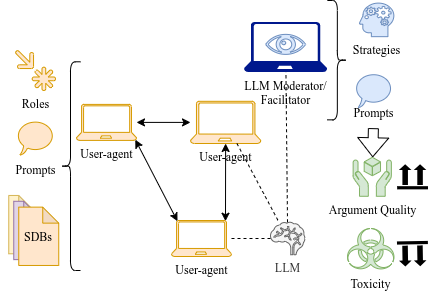
\includegraphics[width=\columnwidth]{research_goal.png}
	\caption{\ac{LLM} user-agents with distinct \acp{SDB} participate in a discussion, while the \ac{LLM} moderator monitors and attempts to improve the quality of the discussion. We need to design prompts and configurations for both types of \ac{LLM} agents.}
	\label{fig::goals}
\end{figure}


A major challenge in connecting facilitation research to real-world needs is    the substantial costs required both in researching and moderating discussions, due to human participation \cite{rossi_2024}. Many social media platforms overcome this by outsourcing moderation to volunteers or their own users \cite{Matias2019TheCL, schaffner_community_guidelines}, while others support only conventional content moderation using traditional \ac{ML} models, which are not enough in practice \cite{horta_automated_moderation, schaffner_community_guidelines}. \acfp{LLM} have been hypothesized to be capable of conversational moderation and facilitation tasks, which often require actively participating in the discussions, instead of passively flagging or removing content \cite{small-polis-llm, korre2025evaluation}. 

While studies exist for simulating user interactions in social media \cite{park_simulacra, mou_2024, tornberg_2023, y_social, balog_2024}, and for using artificial facilitators \cite{kim_et_al_chatbot, cho-etal-2024-language}, none so far have combined the two approaches. We posit that synthetic simulations can be a cheap and easy way to develop and test preliminary, in silico experiments with \ac{LLM} facilitators, initial versions of which may be unstable or unpredictable \cite{atil_2025, rossi_2024}, before testing them in much more costly experiments with human participants. Our work thus asks the following two questions: (1) Can we produce high-quality synthetic discussions, involving alternative facilitation strategies, by crafting an appropriate environment for simulations? (2) Can we boost the effectiveness of \ac{LLM} moderators (in synthetic discussions) by using prompts aligned with facilitation strategies proposed in modern Social Science research?

We propose a simple and generalizable approach using \ac{LLM}-driven synthetic experiments for online moderation research, enabling fast and inexpensive model “debugging” and parameter testing (e.g.,  \ac{LLM} moderator prompts, instructions) without human involvement (\S\ref{sec:methodology}) (Fig.~\ref{fig::goals}). An ablation study (\S\ref{ssec:results:ablation}) demonstrates that each step of our methodology meaningfully contributes to generating high-quality synthetic data. Using this methodology, we examine four \ac{LLM} moderation strategies (including a novel strategy inspired by \ac{RL}) based on current Social Science facilitation research (\S\ref{sec:experimental})
%: \ac{LLM} alignment guidelines \cite{collective_constitution}, prompts based on human facilitation guidelines \cite{Cornell_eRulemaking2017, dimitra-book} and our own prompt based on \ac{RL} (although we do not perform \ac{RL} in this paper). We 
and compare them with two baselines (\ac{LLM} facilitators with simplistic facilitation prompts). \acp{LLM} are also used to gauge discussion quality (e.g., argument quality, toxicity).

Our analysis reveals two key findings (\S\ref{sec:results}): (1) the presence of \ac{LLM} facilitators has a positive and statistically significant influence on the quality of synthetic discussions, and (2) facilitation strategies inspired by Social Science research often do not manage to outperform simpler baselines. %However, besides helping in understanding the effect of prompts to \ac{LLM} moderators, the synthetic data presented in this paper can also be used to finetune them.
Furthermore, we release \syndisco an open-source Python framework for generating and evaluating synthetic discussions, alongside \vmd\datasetlink a large, publicly available dataset comprising automatically evaluated synthetic discussions (\S\ref{sec:data-soft}). %Finally, we outline the limitations (\S\ref{sec:limitations}) and ethical considerations (\S\ref{sec:ethical}) of our work. 
We use open-source \acp{LLM} and include all relevant configurations in order to make our study as reproducible as possible (see \S\ref{ssec:appendix:annotation}, \S\ref{ssec:appendix:prompts}).